\documentclass{article}
\usepackage{graphicx}
\usepackage[margin=1.5cm]{geometry}
\usepackage{amsmath}

\begin{document}
\twocolumn

\title{Wednesday warm-up: displacement, velocity, and acceleration vectors}
\author{Prof. Jordan C. Hanson}

\maketitle

\section{Memory Bank}

\begin{enumerate}
\item $\Delta x = \vec{x}_f - \vec{x}_i$ ... Definition of displacement
\item $\Delta t = t_f - t_i$ ... Definition of time duration
\item $\vec{v} = \Delta \vec{x} / \Delta t$ ... Definition of vector velocity
\item $\vec{a} = \Delta \vec{v} / \Delta t$ ... Definition of vector acceleration
\item $x(t) = \frac{1}{2}at^2 + v_i t + x_i$ ... Displacement, for constant acceleration
\item $v(t) = at + v_i$ ... Velocity, for constant acceleration
\item $a(t) = a$ ... Constant acceleration
\end{enumerate}

\section{Acceleration}

\begin{enumerate}
\item A vehicle with different velocity and \textit{acceleration} vectors is shown in Fig. \ref{fig:vehicle_v_a}.  Match the pictures to the following statements.  (1) The vehicle is moving to the right and speeding up.  (2) The vehicle is moving to the right and slowing down.  (3) The vehicle is moving to the left and speeding up. (4) The vehicle is moving to the left and slowing down. \\ \vspace{0.1cm}
\item Suppose the velocity of the vehicle in Fig. \ref{fig:vehicle_v_a} is 40 km hr$^{-1}$ at $t=0$ seconds, and 80 km hr$^{-1}$ at $t=5$ seconds. (a) What is the acceleration in km hr$^{-1}$ s$^{-1}$? (b) What is the acceleration in m s$^{-2}$? \\ \vspace{2cm}
\end{enumerate}

\section{Kinematics II}

\begin{enumerate}
\item (a) Prove Eq. 6 from Eq. 5 in the Memory Bank. (b) Prove Eq. 7 from Eq. 6 in the Memory Bank. \\ \vspace{2cm}
\item Suppose a racing vehicle begins at the starting line.  At $t = 0$, the driver accelerates with $a=6$ m s$^{-2}$. (a) How long before the vehicle reaches its top speed of 200 km hr$^{-1}$? (b) If it continues at this speed, how long before the vehicle has traveled 0.417 km? \\ \vspace{3cm}
\item Suppose a member of the Whittier College swim team dives from a 5 m height into the pool.  (a) If the downward acceleration is 9.81 m $s^{-2}$, when does she touch the water? (b) What is her speed at that moment? \\ \vspace{2cm}
\item Let $v_f$ and $v_i$ be the velocities at $t_f$ and $t_i$, respectively.  Use the equations in the Memory Bank to show that
\begin{equation}
v_f^2 = v_i^2 + 2 a \Delta x
\end{equation}
\end{enumerate}

\begin{figure}
\centering
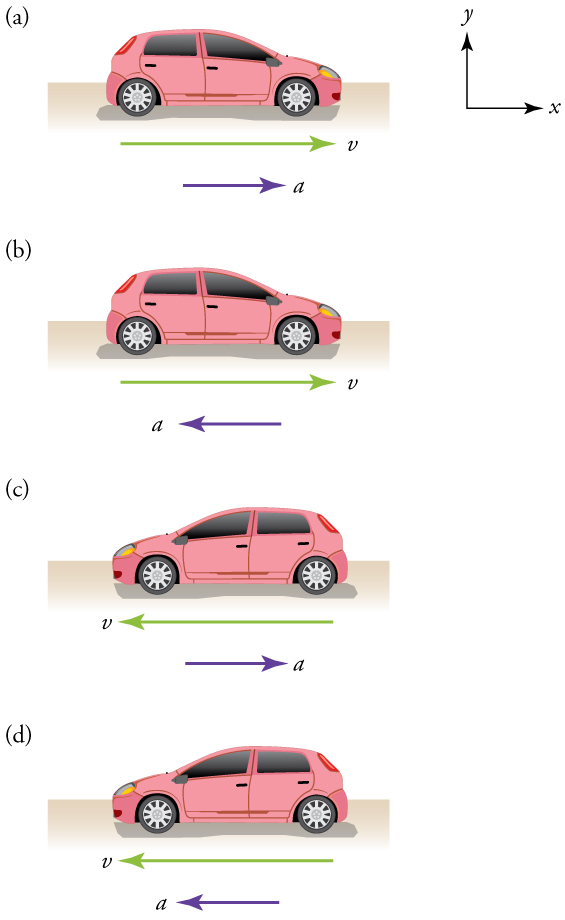
\includegraphics[width=0.17\textwidth,trim=0cm 0cm 1.75cm 0cm,clip=true]{figures/vehicle_v_a.jpeg}
\caption{\label{fig:vehicle_v_a} Four cases of velocity and acceleration in one dimension.}
\end{figure}

\end{document}
